\chapter{Resonator}
Lasering principle in a resonator with laser active medium which achieves population inversion:
\begin{enumerate}
    \item Spontaneous emission $\rightarrow$ incoherent, unpolarized light with random direction, phae, polarization. Wavelength is given by the lifetime of excited state
    \item Spontaneous emission will cause stimulated emission (amplified spontaneous emission ASE)
    \item ASE-light still has the same properties - unpolarized and incoherent 
\end{enumerate}
To get a better coherence, a \textit{feedback} mechanism is required - we use a \textbf{resonator}.
Mirrors feed back spontaneous emission and ASE to the laser medium and select a certain propagation direction.
Show on figure \ref{fig:res1}. We assume that the inverse population is kept by continuous laser pumping. Light reflected from the mirrors causes stimulated emission. Light with direction unsuported by mirrors leaves the resonator,
stimulated emission amplifies the \textit{allowed} directions over several cycles. 

\begin{figure}[h!]
    \centering
    \includegraphics[width=0.5\textwidth]{slike/res1.pdf}
    \caption{Simple resonator}
    \label{fig:res1}
\end{figure}

\textbf{Laser resonator}:
\begin{itemize}
    \item Intensity of light propagating in supported direction by resonator mirrors increases very fast 
    \item Propagation direction inside the laser resonator is fixed
    \item Incidence angles are fixed
    \item \textbf{Polarization with the smallest losses and largest gain wins}
    \item Time bandwidth product drops to its minimal possible value
\end{itemize}

\section{Spectral properties}
In a resonator only a standing waves with integer number $q$ of half-wavelength are possible.
Number $q$ depends on length of a resonator $L$ and $lambda$ - equation \ref{eq:res1}.
\begin{equation}
    L = q \cdot \frac{\lambda}{2}
    \label{eq:res1}
\end{equation}
Frequency separation between modes is calculated by the equation \ref{eq:res2}.
\begin{equation}
    \Delta \nu = \frac{c}{2 n L}
    \label{eq:res2}
\end{equation}
Where $n$ is the average index of refraction in a resonator. 
Figure \ref{fig:resmodes} show longitudinal modes in a resonator.
\begin{figure}[h!]
    \centering
    \includegraphics[width=0.5\textwidth]{slike/modes.pdf}
    \caption{Modes in a resonator}
    \label{fig:resmodes}
\end{figure}
Frequency separation is shown on figure \ref{fig:freqsep}.
\begin{figure}[h!]
    \centering
    \includegraphics[width=0.5\textwidth]{slike/deltalambda.pdf}
    \caption{$\Delta \lambda$ and $\Delta \nu$ }
    \label{fig:freqsep}
\end{figure}

\section{Time-bandwidth product of a laser resonator}

We know that in resonator, only certain frequency are allowed and that real resonators have losses, due to imperfections
in the mirrors. In the ideal case, we can get the time-bandwidth product from the frequency bandwidth from the extents (razsežnosti), which are given by the time duration of the photons ($\tau$)?????

%what are extents??

\section{Losses}
Figure \ref{fig:schres} show a simplified resonator. 
\begin{figure}
    \centering
    \includegraphics[width=0.5\textwidth]{slike/resonator_losses.pdf}
    \caption{Lossy resonator}
    \label{fig:schres}
\end{figure}
We calculate \textit{one round trip} losses with equation \ref{eq:losses}. Constants and variables are shown in table \ref{tab:losses}.
\begin{equation}
    R_1 R_2 e^{2 \alpha_m L_m} = e^{-2 \alpha_m L_m + ln(R_1 R-2)} = e^{2 \alpha_r L_R}
    \label{eq:losses}
\end{equation}

\begin{table}[h!]
    \centering
    \begin{tabular}{|l|p{2in}|}
        \hline
        $R$ & Mirror reflectivity \\
        $\alpha_m$ & Losses in gain medium \\
        $L_m$ & Gain medium length\\
        $L_R$  & Resonator length \\
        \hline
    \end{tabular}
    \caption{Constants}
    \label{tab:losses}
\end{table} 
For a free space resonator $\alpha_m L_m << 1$, $R_1 R_2 e^{2 \alpha_m L_m} \approx R_1 R_2 \cdot 1 =  e^{2 \alpha_r L_R}$, from which  we get 
$\alpha_r = -\frac{ln(R_1 R_2)}{2 L_R}$.
Time dependant energy loss in a resonator can be expressed as $E(t) = E_0 \cdot e^{\alpha_r c t}$. Distance $x$ is a $x_P = x \tau = \frac{1}{\alpha_r}$ is the characteristic propagation length.
Time $\tau$ is a lifetime unit of a photon in the resonator, calculated as $\tau_P = \frac{1}{\alpha_r \cdot c}$.

Resonator line width is $\delta \nu = \frac{1}{2 \pi \tau_P}$

\section{Resonator with laser active medium}
Laser emits radiation in a comb of discrete frequencies, for a majority of applications, lasers can be 
treated as monochromatic radiation sources. Exceptions are interferometric applications, such as holographic systems or ultrafast lasers.
Figure \ref{fig:lamr} show the possible frequencies in a laser resonator with laser active medium.

\begin{figure}[h!]
    \centering
    \includegraphics[width=0.3\textwidth]{slike/activemediumresonator.pdf}
    \caption{Laser output spectrum}
    \label{fig:lamr}
\end{figure}

Laser oscillations can only be build-up for modes satisfying gain $G > 1$ for the condition \ref{eq:Gainresonator}.
\begin{equation}
    G = R_1 R_2 e^{2(g(\nu) - \alpha) L_m} \ge 1
    \label{eq:Gainresonator}
\end{equation}
Where $g(\nu)$ is a gain coefficient, which is a function of frequency $\nu$.
Gain factor is show in figure \ref{fig:gainfunc}.
\begin{figure}[h!]
    \centering
    \includegraphics[width=0.4\textwidth]{slike/gainfunc.pdf}
    \caption{Gain function}
    \label{fig:gainfunc}
\end{figure}

\section{Stability of resonators}
Resonator can be:
\begin{table}[h!]
    \begin{tabular}{l p{5in}}
        stable & light does not leave resonator after infinite number of reflections\\
        unstable & light leaves resonator after a certain number of reflections
    \end{tabular}
\end{table}

Figure \ref{fig:resstab} shows stable and unstable resonator.
\begin{figure}[h!]
    \centering
    \includegraphics[width=0.5\textwidth]{slike/typres.pdf}
    \caption{Stable and unstable resonator}
    \label{fig:resstab}
\end{figure}

Stable resonator will have a shorter bandwidth. Resonator is described by parameters shown in table \ref{tab:resparms}. Shown on figure 
\ref{fig:resstab}.
\begin{table}[h!]
    \centering
    \begin{tabular}{|l| p{2in}|}
        \hline
        L & mirror separation \\
        $r_i$ & mirror radius of curvature\\
        $d_{s1}$ & mirror diameter \\
        \hline
    \end{tabular}
    \caption{Resonator parameters}
    \label{tab:resparms}
\end{table}

\subsection{Resonator Configuration}
Resonator configurations, shown on figure \ref{fig:resconf}, influence resonator stablility.
\begin{figure}[h!]
    \centering
    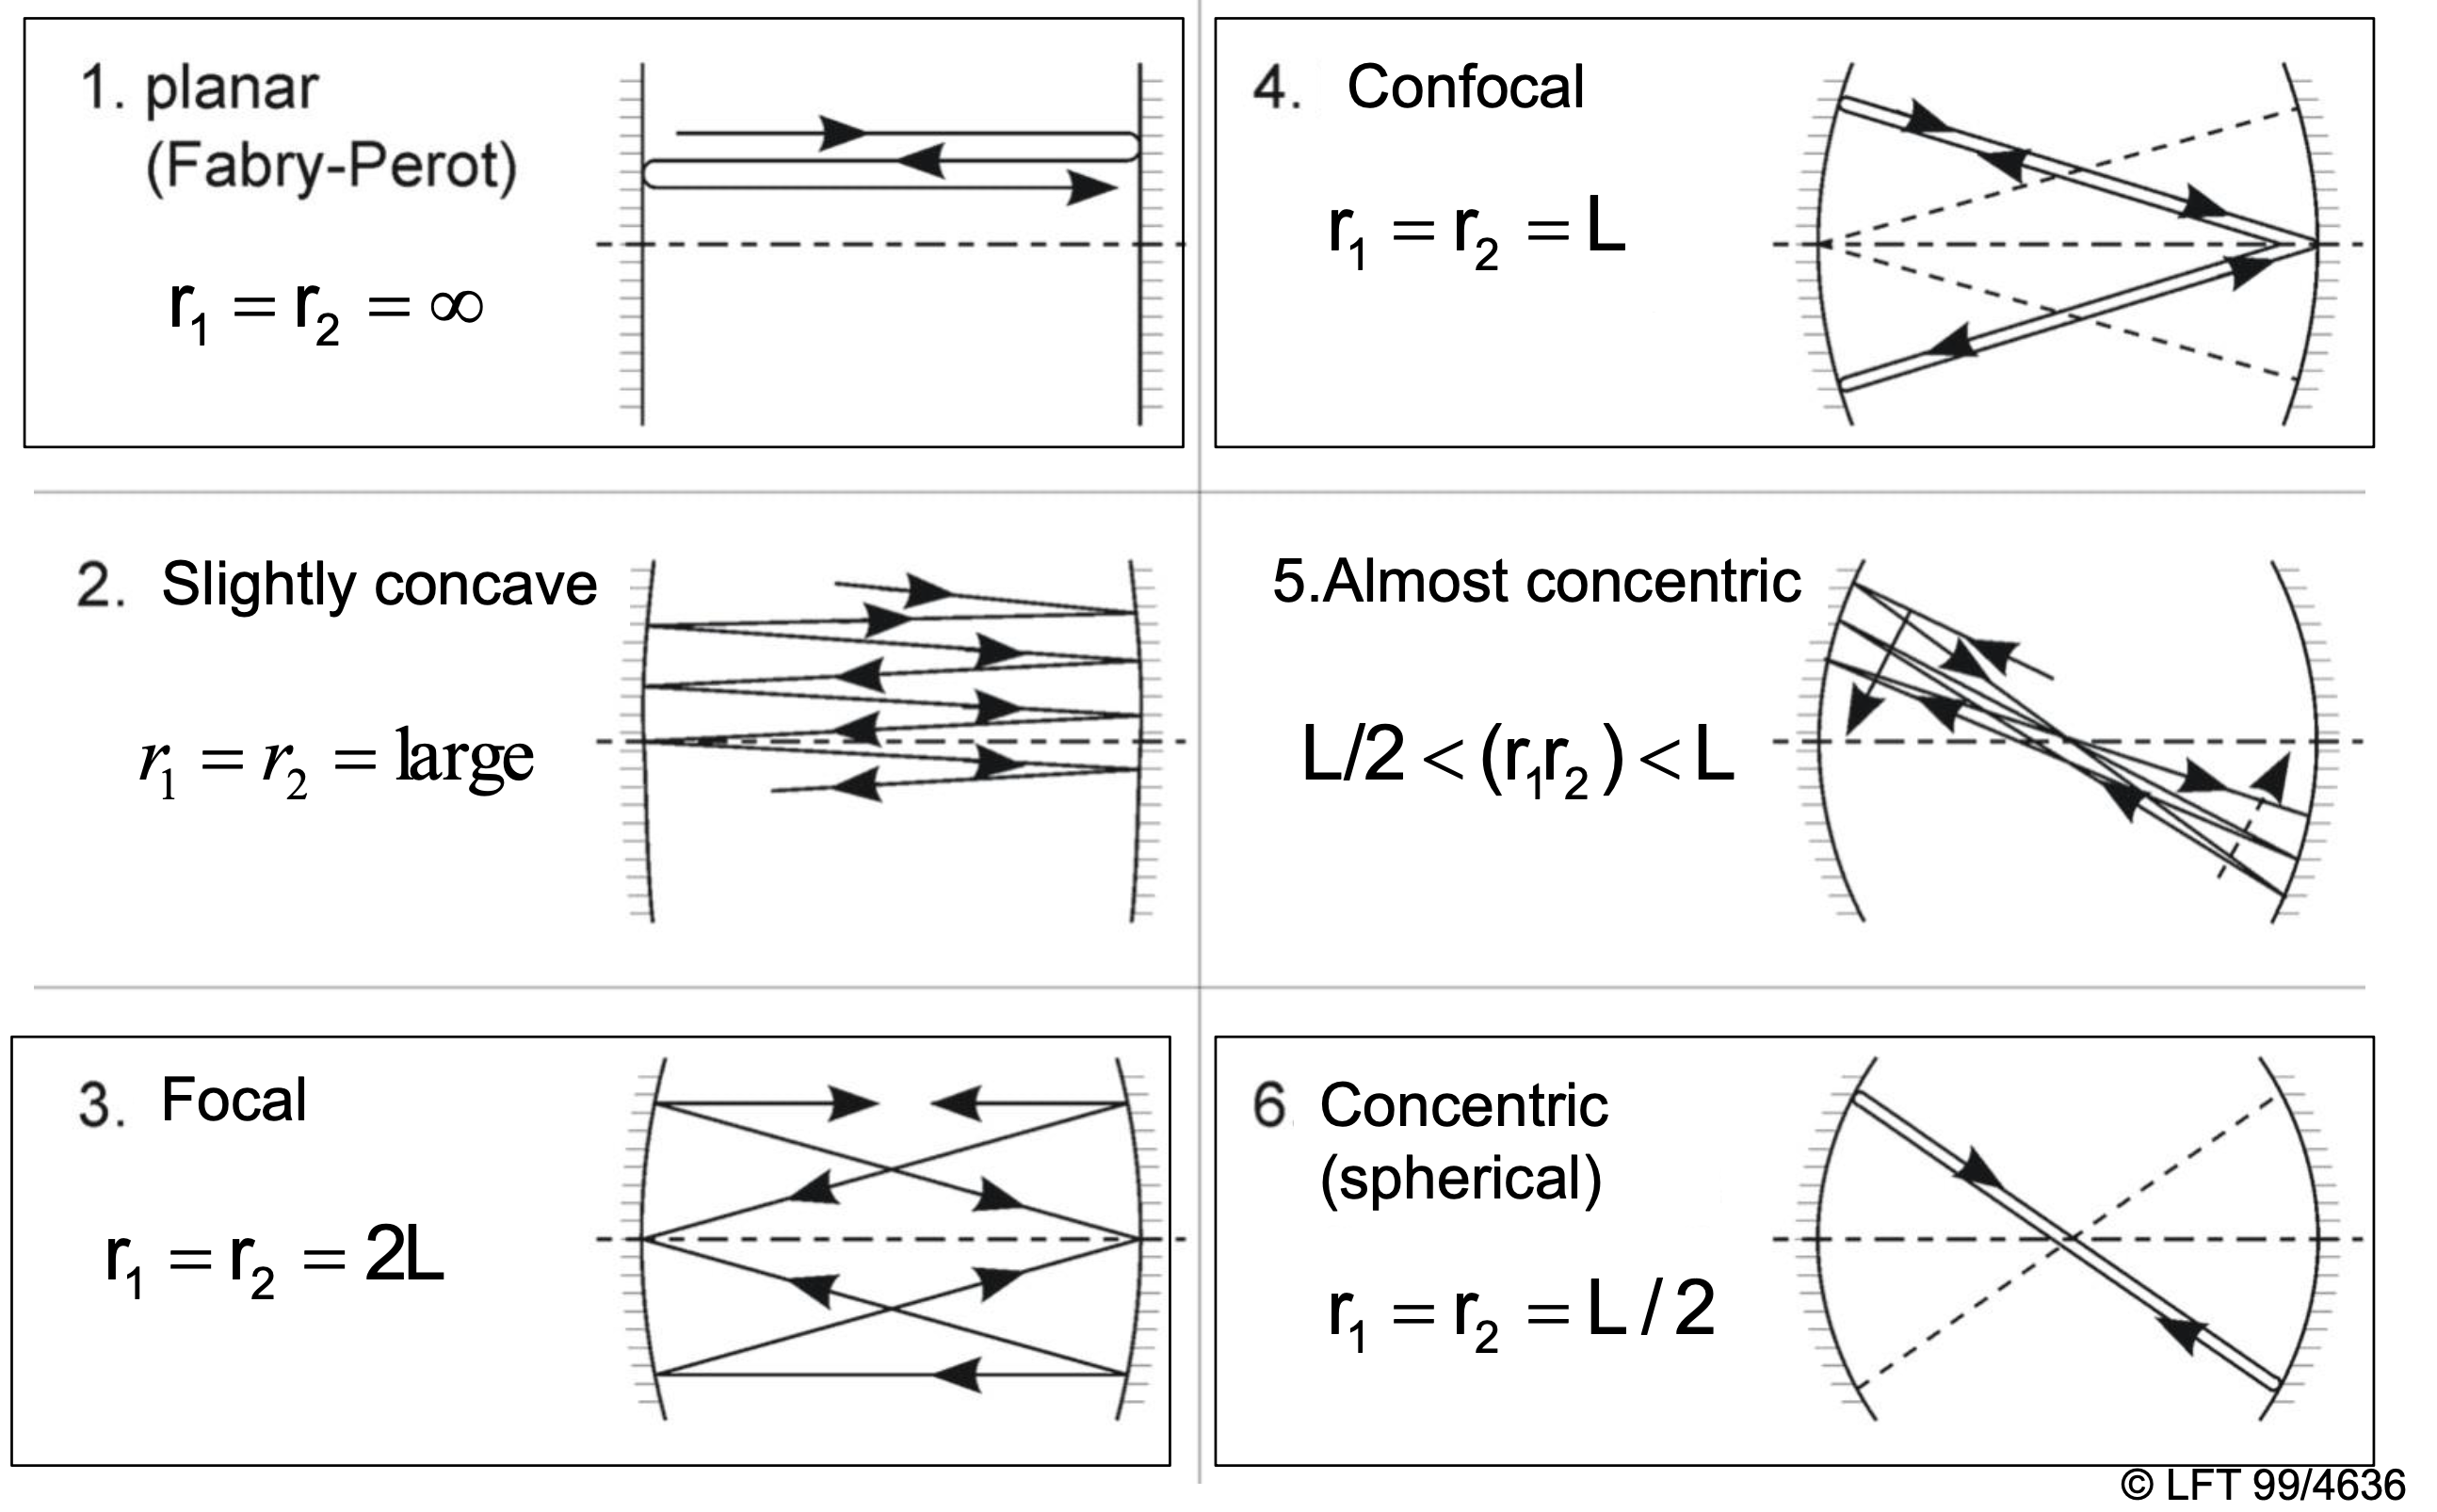
\includegraphics[width=0.75\textwidth]{slike/res_configs.png}
    \caption{Resonator configuration. \textit{Source: lecture notes} }
    \label{fig:resconf}
\end{figure}
To describe the resonator, we can use the \textit{general (ABCD matrix)} or a \textit{simplified approach (g-parameters)}.
General approach is necessary for free space beam propagation, compared to g-parameters, it is more computaionaly expensive.
Simplified approach can only be used for two mirror resonators.

\subsubsection{Generalized approach}
Generalized approach - ABDC matrix formalism or raytracing is an approach that we use on more complex resonators - more than \textit{two mirrors}.

Mirrors can be described as lenses, simply by switching to a suitable coordinate system. To describe an optical beam or ray at any position,
we can use its position $x$ and its angle to optical axis $\alpha$. State of beam is therefore given by a vector $\begin{pmatrix}
    x\\ \alpha \end{pmatrix}$.



Beam propagation through mirror/lens consists of three steps:
\begin{table}[h!]
    \centering
    \begin{tabular}{|p{2in}|p{2in}|p{2in}|}
       \hline
        Propagation through \textit{air} \newline(parameter: distance) &
         Propagation through \textit{mirror/lens}\newline (parameter: focal length) & 
         Propagation through \textit{air}\newline (parameter: distance)\\
        \hline
    \end{tabular}
\end{table}
Effects of lens or mirror on a beam are shown of figure \ref{fig:eff}.
\begin{figure}[h!]
    \centering
    \includegraphics[width=0.9\textwidth]{slike/lenseff2.pdf}
    \caption{Effect of  lens/mirror}
    \label{fig:eff}
\end{figure}
Beam angle changes depending on focal length $f$, on position $x$ at which the beam arrives at the lens and the angle that a beam has
in front of the lens $\alpha_{in}$.
For center ray - blue line on figure \ref{fig:eff} - the beam leaves the lens at the same position, $x_{in} = x_{out}$, but the beam angle $\alpha$ changes.
Change of $\alpha$ depends on:
\begin{itemize}
    \item focal length $f$
    \item on position $x$ at which the beam arrives at the lens
    \item on the initial $\alpha_{in}$ in front of the lens 
\end{itemize}
Exiting angle $\alpha_{out}$ is calculated by the equation \ref{eq:aout}.
\begin{equation}
    \alpha_{out} = -\frac{x_{in}}{f} + \alpha_{in}
    \label{eq:aout}  
\end{equation}
Position of exiting beam changes according to the input angle $\alpha_{in}$ and propagation distance $L$, equation \ref{eq:xout}.
\begin{equation}
    x_{out} = x_{in} + L \cdot \alpha_{in}
    \label{eq:xout}
\end{equation} 

To simplify the notation, we can use matrices.
Beam propagation \textbf{through air}, can be written as shown in equation \ref{eq:mair}.
\begin{equation}
    \begin{pmatrix}
        x_{out} \\ \alpha_{out}
    \end{pmatrix} = \begin{pmatrix}
        x_{in} + L \alpha_{in} \\ \alpha_{in}
    \end{pmatrix} = \begin{pmatrix}
        1 & L \\ 0 & 1
    \end{pmatrix} \begin{pmatrix}
        x_{in} \\ \alpha_{in}
    \end{pmatrix}
    \label{eq:mair}
\end{equation}
Propagation \textbf{through mirror/lens}, can be wirtten as equation \ref{eq:mlens}.
\begin{equation}
    \begin{pmatrix}
        x_{out} \\ \alpha_{out}
    \end{pmatrix} =     \begin{pmatrix}
        x_{in} \\ -\frac{x_{in}}{f} \alpha_{in}
    \end{pmatrix}  = \begin{pmatrix}
        1 & 0 \\ -f^{-1} & 0
    \end{pmatrix} \begin{pmatrix}
        x_{in} \\ \alpha_{in}
    \end{pmatrix}
    \label{eq:mlens}
\end{equation}
Where $f_{mirror}$ is equal to $\frac{R_{mirror}}{2}$.


\textbf{ABCD formalism}

In equations \ref{eq:mair} and \ref{eq:mlens} we have defined two matrices. A matrix for free space propagation and a matrix for 
lens/mirror. 
Free space propagation matrix, shown in \ref{eq:fspm} and a matrix for lens/mirror propagation, shown in \ref{eq:mlpm}.
\begin{equation}
    P(L) =\begin{pmatrix}
        1 & L \\ 0 & 1
    \end{pmatrix}
    \label{eq:fspm}
\end{equation}

\begin{equation}
    M(f) = \begin{pmatrix}
        1 & 0 \\ -\frac{1}{f} & 0
    \end{pmatrix}
\label{eq:mlpm}
\end{equation}

Each path can be described as a multiplication of matrices, in the reverse order of light propagation, as shown in figure \ref{fig:abcdl}.
\begin{figure}[h!]
    \centering
    \includegraphics[width=0.7\textwidth]{slike/ABCD_lens.pdf}
    \caption{Propagation description by matrix multiplication}
    \label{fig:abcdl}
\end{figure}

Propagation inside the resonator can be simplified further - path is always the same, so we can introduce a new matrix $R$,
which is equal to the path of the light, for example for a resonator mirror-air-mirror-air, path  can be written as $R = P \cdot M_2 \cdot P \cdot M_1$.
For each cycle the light makes, we multiply the matrix $R$ by its self - equation \ref{eq:path}.
\begin{equation}
    \begin{pmatrix}
        x_{out} \\ \alpha_{out}
    \end{pmatrix} = R^n \cdot \begin{pmatrix}
        x_{in} \\ \alpha_{in}
    \end{pmatrix} = \prod_{1}^{n} R \cdot \begin{pmatrix}
        x_{in} \\ \alpha_{in}
    \end{pmatrix}
    \label{eq:path}
\end{equation}
\textit{Note: in $R^n$ is not exponent, but the amount of multiplications!}\\

For true resonator stability $n$ should be able to go to infinity without increasing the output postion or output angle.
Stability for a single cycle is calculated by the equation \ref{eq:ssc}.
\begin{equation}
    \vec{b}_{out} = R \cdot \vec{b}_{in} = \lambda \cdot  \vec{b}_{in}
    \label{eq:ssc}
\end{equation}
Beam parameter $b$ is the eingenvector of matrix $R$, $\lambda$ is the eigenvalue of matrix $R$,$0 \le \lambda \le 1$.
We can also state: $R \cdot \vec{b} = \lambda \cdot \vec{b}$.

To find the eigenvalues of in problems such as $R \cdot \vec{b} = \lambda \cdot \vec{b}$, we can find both eigen values $\lambda_{\pm}$ by solving the equation \ref{eq:eigval}.
\begin{equation}
    \lambda_{\pm} = \frac{A + D}{2} \pm \sqrt{(\frac{A+D}{2})^2 - det(R)}
    \label{eq:eigval}
\end{equation}
Where $R = \begin{pmatrix}
    A & B \\ C&D
\end{pmatrix}$. In case the resonator only consist of two mirrors, we derive the simpified approach.

\subsubsection{Simplified approach}
In case of resonator with only two mirrors, we can calculate the stability by equation \ref{eq:sr1}.
\begin{equation}
    0 \le g_1 g_2 \le 1
    \label{eq:sr1}
\end{equation}
Where $g_1 = 1 - \frac{1}{R_1}$ and $g_2 = 1 - \frac{1}{R_2}$, $R_i$ is the mirror curvature.
\newpage
Stability of a simplified resonator is shown in figure \ref{fig:slr}.
\begin{figure}[h!]
    \centering
    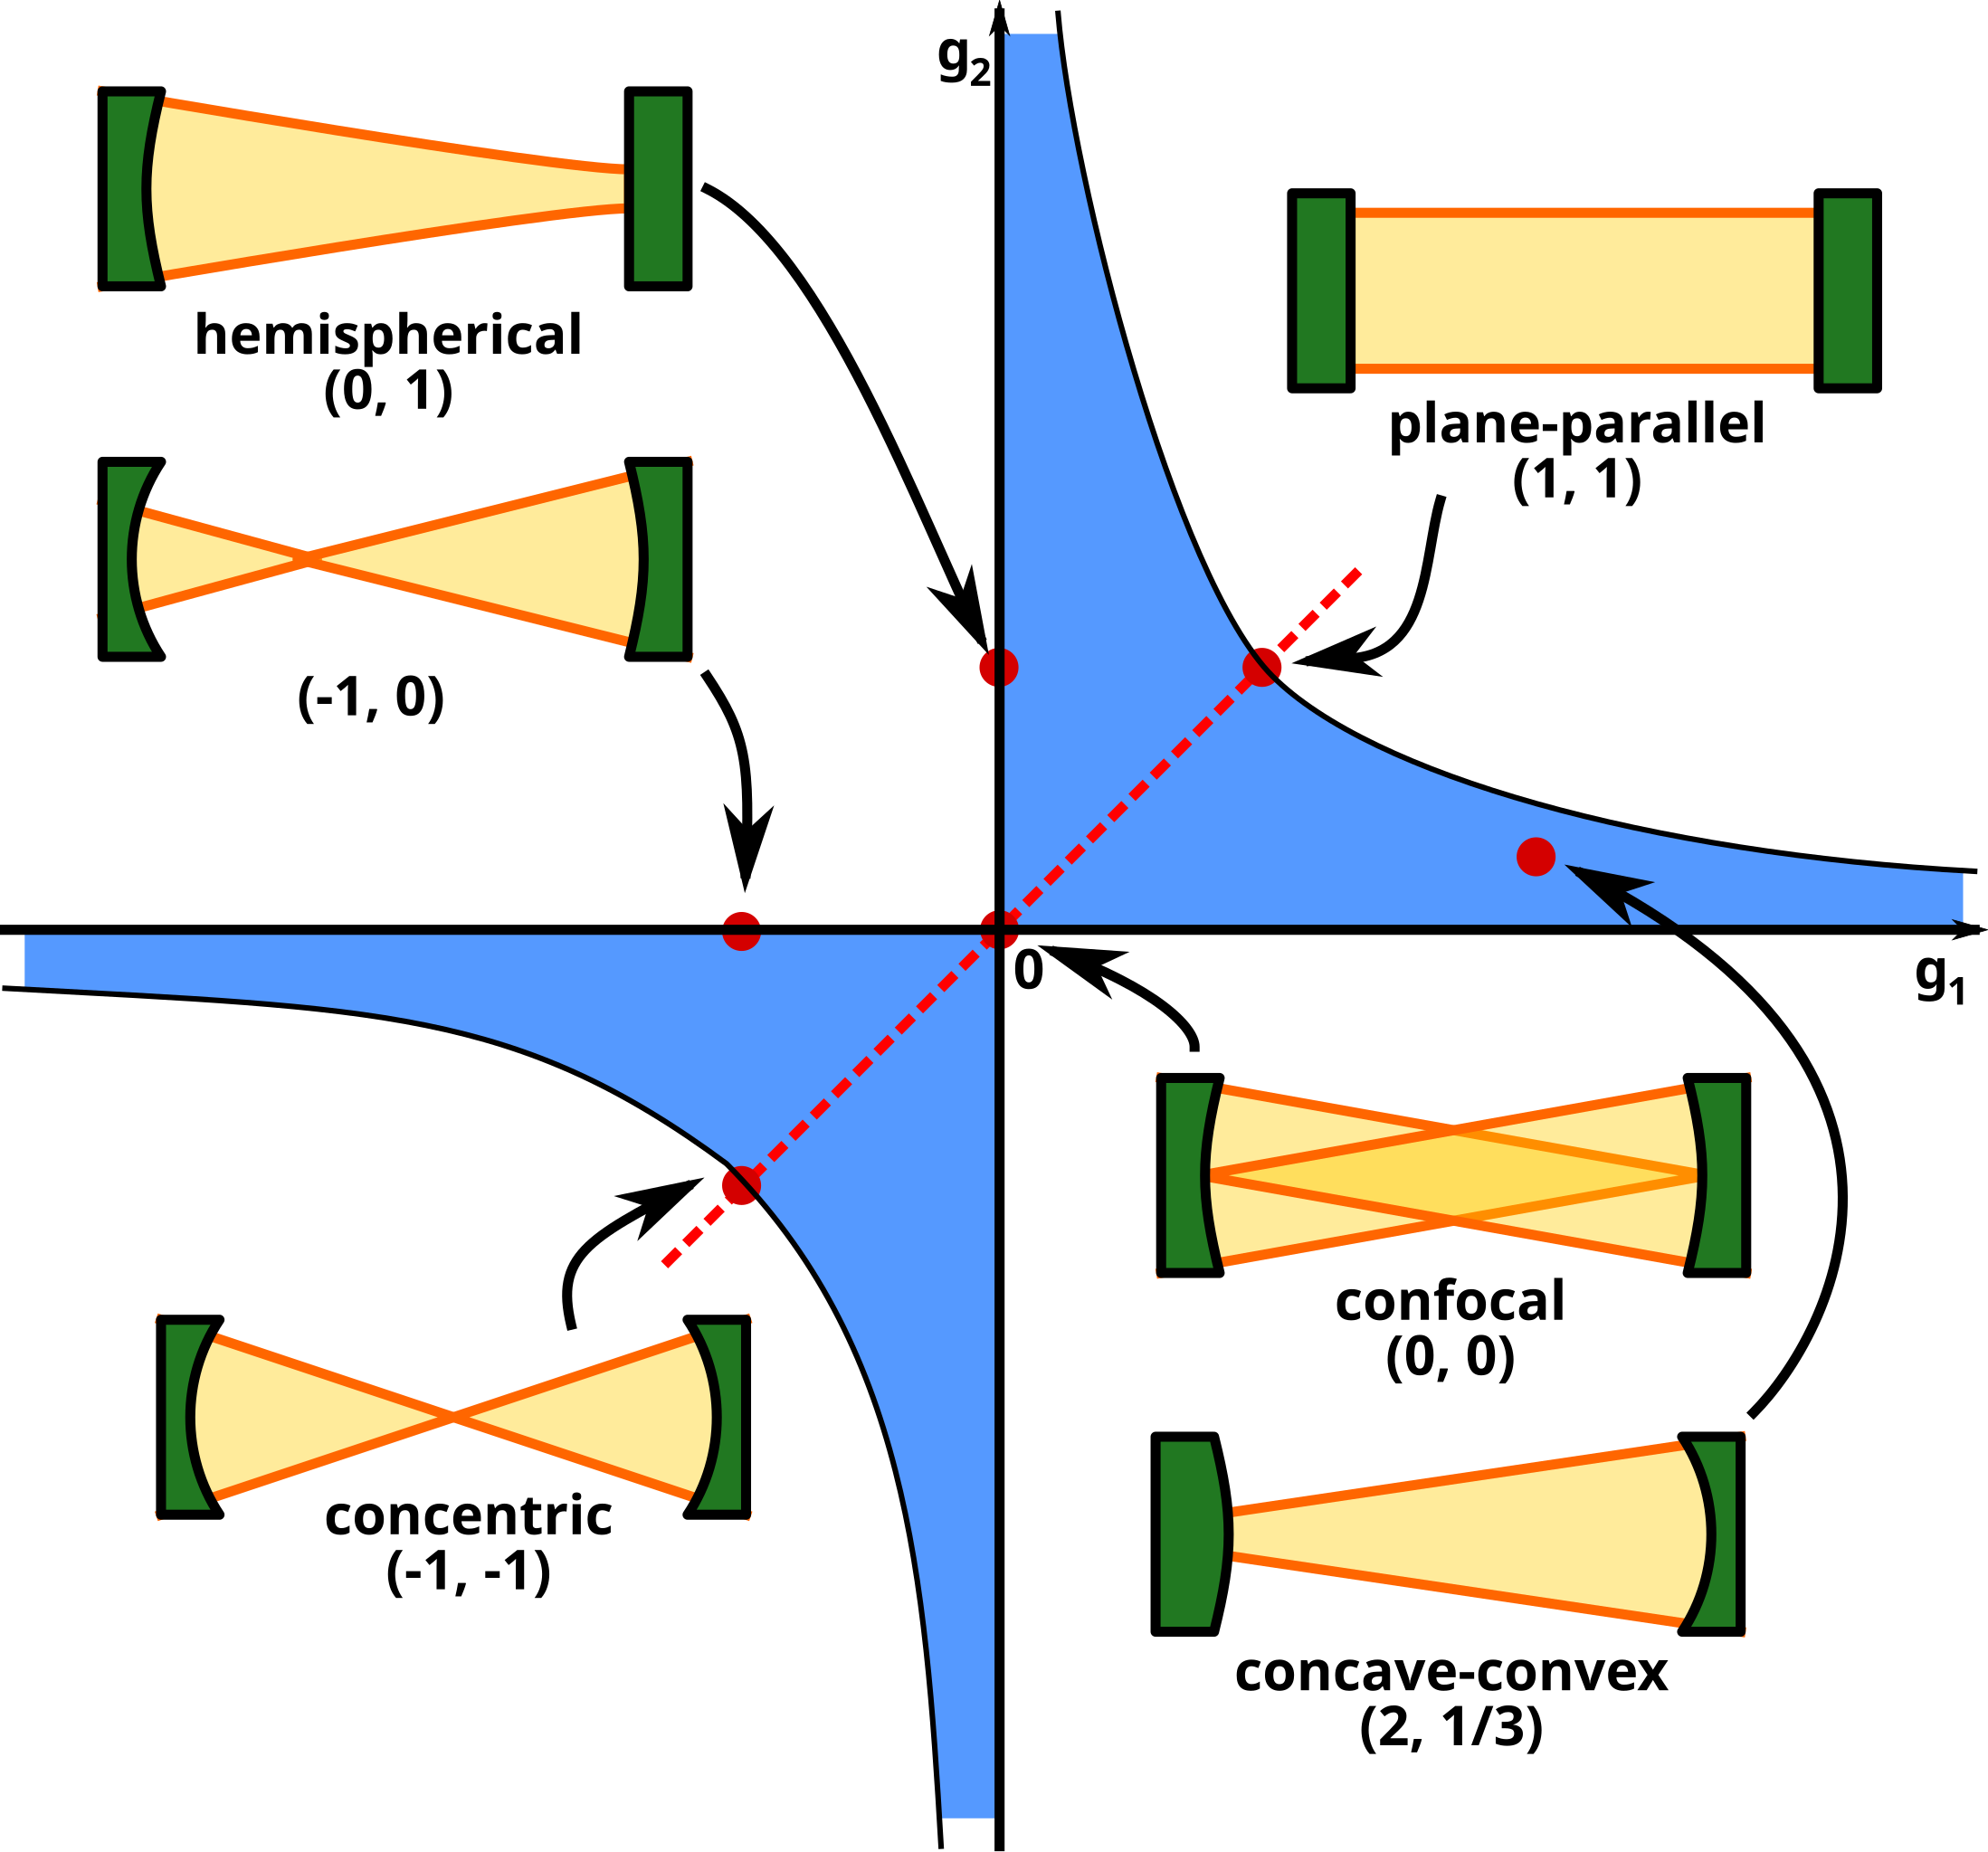
\includegraphics[width=0.5\textwidth]{slike/Laser_resonator_stability.png}
    \caption{Resonator stability}
    \label{fig:slr}
\end{figure}

We can use both \textbf{stable} and \textbf{unstable} resonators, stable resonator provide small beam parameter product and good beam quality.
Unstable resonators provide large beam parameter product, their advantage is, that they do not require a transmissive element.